\section{Gitting started}	% huehue

\subsection{Repository aanmaken}
\begin{frame}[fragile]
	%\frametitle{Repository aanmaken}
	\begin{enumerate}
		\item Open terminal (windows: \alert{git-bash})
		\item \texttt{cd} naar map die je wil bijhouden
			(of \texttt{mkdir} een nieuwe)
		\item \texttt{git init}
		\item \texttt{git status}
	\end{enumerate}
	Als het goed is zie je nu \alert{niet}:
	\begin{minted}{text}
fatal: Not a git repository or 
	any of the parent directories: .git
	\end{minted}
\end{frame}

\subsection{Bestanden laten bijhouden}
\begin{frame}[fragile]
	\begin{enumerate}
		\item \texttt{git status}
		\item Bekijk 'untracked files'
		\item \texttt{git add bestand1 bestand2 map1}\\ of:
			\texttt{git add .}\\
			(map pakt alle bestanden erin mee, . is huidige map)
		\item \texttt{git commit}, voer bericht in, opslaan en sluiten\\
			(of: \texttt{git commit -m "Eerste commit"})
	\end{enumerate}
	Resultaat: 
	\begin{minted}{text}
	[master 1234abc] Eerste commit
	x files added
	\end{minted}
\end{frame}

\frame{
	\begin{center}
		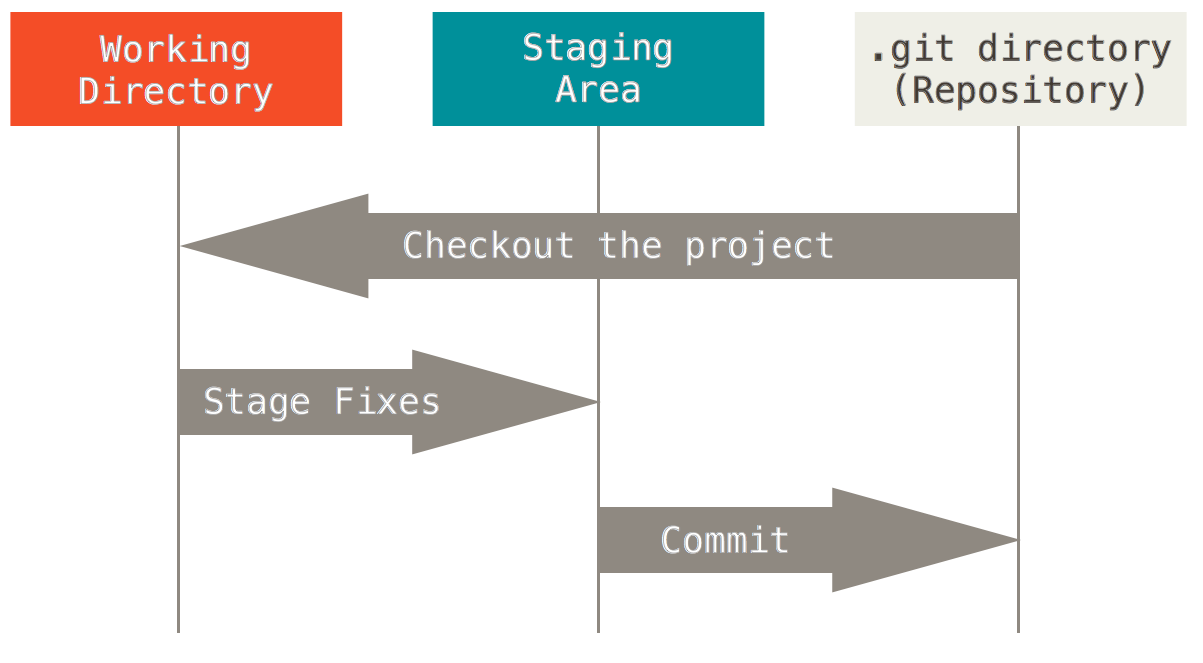
\includegraphics[width=\textwidth]{images/areas}
	\end{center}
	\begin{itemize}
		\item \texttt{git add} $\rightarrow$ 'Stage Fixes'
		\item \texttt{git commit} $\rightarrow$ 'Commit'
	\end{itemize}
}

\subsubsection{Bestanden negeren}
\begin{frame}[fragile]{Bestanden negeren}
	\begin{enumerate}
		\item \texttt{git status} geeft onbekende bestanden altijd aan
		\item Oplossing: \texttt{.gitignore}:
	\end{enumerate}
	\begin{minted}{text}
		# alle bestanden in de map bin
		bin/*

		# alle .exe
		*.exe

		# maar wel dinges.exe
		!dinges.exe
	\end{minted}
\end{frame}

\subsection{Wat is er gebeurd?}
% git log
\begin{frame}{log}
	\begin{tabular}{ll}
		\texttt{git log}& Bekijk geschiedenis van commits (\texttt{--reverse}: oudste eerst)\\
		\texttt{git show}& Bekijk veranderingen in 1 commit, standaard de nieuwste
	\end{tabular}
\end{frame}

% git diff
\begin{frame}{git diff}
	\begin{tabular}{ll}
		\texttt{git diff}&Toon veranderingen in tracked files (unstaged)\\
		\texttt{git diff --staged}&Toon veranderingen klaargezet voor commit\\
		\texttt{git diff HEAD\^}&Toon veranderingen sinds vorige commit
	\end{tabular}
\end{frame}

% git show
\begin{frame}{git show}
	\begin{tabular}{ll}
		\texttt{git show}&Toon info over vorige commit\\
		\texttt{git show id}&Toon info over commit \texttt{id}\\
	\end{tabular}
\end{frame}
